% Options for packages loaded elsewhere
\PassOptionsToPackage{unicode}{hyperref}
\PassOptionsToPackage{hyphens}{url}
%
\documentclass[
  man]{apa7}
\usepackage{amsmath,amssymb}
\usepackage{lmodern}
\usepackage{iftex}
\ifPDFTeX
  \usepackage[T1]{fontenc}
  \usepackage[utf8]{inputenc}
  \usepackage{textcomp} % provide euro and other symbols
\else % if luatex or xetex
  \usepackage{unicode-math}
  \defaultfontfeatures{Scale=MatchLowercase}
  \defaultfontfeatures[\rmfamily]{Ligatures=TeX,Scale=1}
\fi
% Use upquote if available, for straight quotes in verbatim environments
\IfFileExists{upquote.sty}{\usepackage{upquote}}{}
\IfFileExists{microtype.sty}{% use microtype if available
  \usepackage[]{microtype}
  \UseMicrotypeSet[protrusion]{basicmath} % disable protrusion for tt fonts
}{}
\makeatletter
\@ifundefined{KOMAClassName}{% if non-KOMA class
  \IfFileExists{parskip.sty}{%
    \usepackage{parskip}
  }{% else
    \setlength{\parindent}{0pt}
    \setlength{\parskip}{6pt plus 2pt minus 1pt}}
}{% if KOMA class
  \KOMAoptions{parskip=half}}
\makeatother
\usepackage{xcolor}
\usepackage{graphicx}
\makeatletter
\def\maxwidth{\ifdim\Gin@nat@width>\linewidth\linewidth\else\Gin@nat@width\fi}
\def\maxheight{\ifdim\Gin@nat@height>\textheight\textheight\else\Gin@nat@height\fi}
\makeatother
% Scale images if necessary, so that they will not overflow the page
% margins by default, and it is still possible to overwrite the defaults
% using explicit options in \includegraphics[width, height, ...]{}
\setkeys{Gin}{width=\maxwidth,height=\maxheight,keepaspectratio}
% Set default figure placement to htbp
\makeatletter
\def\fps@figure{htbp}
\makeatother
\setlength{\emergencystretch}{3em} % prevent overfull lines
\providecommand{\tightlist}{%
  \setlength{\itemsep}{0pt}\setlength{\parskip}{0pt}}
\setcounter{secnumdepth}{-\maxdimen} % remove section numbering
% Make \paragraph and \subparagraph free-standing
\ifx\paragraph\undefined\else
  \let\oldparagraph\paragraph
  \renewcommand{\paragraph}[1]{\oldparagraph{#1}\mbox{}}
\fi
\ifx\subparagraph\undefined\else
  \let\oldsubparagraph\subparagraph
  \renewcommand{\subparagraph}[1]{\oldsubparagraph{#1}\mbox{}}
\fi
\newlength{\cslhangindent}
\setlength{\cslhangindent}{1.5em}
\newlength{\csllabelwidth}
\setlength{\csllabelwidth}{3em}
\newlength{\cslentryspacingunit} % times entry-spacing
\setlength{\cslentryspacingunit}{\parskip}
\newenvironment{CSLReferences}[2] % #1 hanging-ident, #2 entry spacing
 {% don't indent paragraphs
  \setlength{\parindent}{0pt}
  % turn on hanging indent if param 1 is 1
  \ifodd #1
  \let\oldpar\par
  \def\par{\hangindent=\cslhangindent\oldpar}
  \fi
  % set entry spacing
  \setlength{\parskip}{#2\cslentryspacingunit}
 }%
 {}
\usepackage{calc}
\newcommand{\CSLBlock}[1]{#1\hfill\break}
\newcommand{\CSLLeftMargin}[1]{\parbox[t]{\csllabelwidth}{#1}}
\newcommand{\CSLRightInline}[1]{\parbox[t]{\linewidth - \csllabelwidth}{#1}\break}
\newcommand{\CSLIndent}[1]{\hspace{\cslhangindent}#1}
\ifLuaTeX
\usepackage[bidi=basic]{babel}
\else
\usepackage[bidi=default]{babel}
\fi
\babelprovide[main,import]{english}
% get rid of language-specific shorthands (see #6817):
\let\LanguageShortHands\languageshorthands
\def\languageshorthands#1{}
% Manuscript styling
\usepackage{upgreek}
\captionsetup{font=singlespacing,justification=justified}

% Table formatting
\usepackage{longtable}
\usepackage{lscape}
% \usepackage[counterclockwise]{rotating}   % Landscape page setup for large tables
\usepackage{multirow}		% Table styling
\usepackage{tabularx}		% Control Column width
\usepackage[flushleft]{threeparttable}	% Allows for three part tables with a specified notes section
\usepackage{threeparttablex}            % Lets threeparttable work with longtable

% Create new environments so endfloat can handle them
% \newenvironment{ltable}
%   {\begin{landscape}\centering\begin{threeparttable}}
%   {\end{threeparttable}\end{landscape}}
\newenvironment{lltable}{\begin{landscape}\centering\begin{ThreePartTable}}{\end{ThreePartTable}\end{landscape}}

% Enables adjusting longtable caption width to table width
% Solution found at http://golatex.de/longtable-mit-caption-so-breit-wie-die-tabelle-t15767.html
\makeatletter
\newcommand\LastLTentrywidth{1em}
\newlength\longtablewidth
\setlength{\longtablewidth}{1in}
\newcommand{\getlongtablewidth}{\begingroup \ifcsname LT@\roman{LT@tables}\endcsname \global\longtablewidth=0pt \renewcommand{\LT@entry}[2]{\global\advance\longtablewidth by ##2\relax\gdef\LastLTentrywidth{##2}}\@nameuse{LT@\roman{LT@tables}} \fi \endgroup}

% \setlength{\parindent}{0.5in}
% \setlength{\parskip}{0pt plus 0pt minus 0pt}

% Overwrite redefinition of paragraph and subparagraph by the default LaTeX template
% See https://github.com/crsh/papaja/issues/292
\makeatletter
\renewcommand{\paragraph}{\@startsection{paragraph}{4}{\parindent}%
  {0\baselineskip \@plus 0.2ex \@minus 0.2ex}%
  {-1em}%
  {\normalfont\normalsize\bfseries\itshape\typesectitle}}

\renewcommand{\subparagraph}[1]{\@startsection{subparagraph}{5}{1em}%
  {0\baselineskip \@plus 0.2ex \@minus 0.2ex}%
  {-\z@\relax}%
  {\normalfont\normalsize\itshape\hspace{\parindent}{#1}\textit{\addperi}}{\relax}}
\makeatother

% \usepackage{etoolbox}
\makeatletter
\patchcmd{\HyOrg@maketitle}
  {\section{\normalfont\normalsize\abstractname}}
  {\section*{\normalfont\normalsize\abstractname}}
  {}{\typeout{Failed to patch abstract.}}
\patchcmd{\HyOrg@maketitle}
  {\section{\protect\normalfont{\@title}}}
  {\section*{\protect\normalfont{\@title}}}
  {}{\typeout{Failed to patch title.}}
\makeatother

\usepackage{xpatch}
\makeatletter
\xapptocmd\appendix
  {\xapptocmd\section
    {\addcontentsline{toc}{section}{\appendixname\ifoneappendix\else~\theappendix\fi\\: #1}}
    {}{\InnerPatchFailed}%
  }
{}{\PatchFailed}
\keywords{keywords\newline\indent Word count: X}
\DeclareDelayedFloatFlavor{ThreePartTable}{table}
\DeclareDelayedFloatFlavor{lltable}{table}
\DeclareDelayedFloatFlavor*{longtable}{table}
\makeatletter
\renewcommand{\efloat@iwrite}[1]{\immediate\expandafter\protected@write\csname efloat@post#1\endcsname{}}
\makeatother
\usepackage{csquotes}
\makeatletter
\renewcommand{\paragraph}{\@startsection{paragraph}{4}{\parindent}%
  {0\baselineskip \@plus 0.2ex \@minus 0.2ex}%
  {-1em}%
  {\normalfont\normalsize\bfseries\typesectitle}}

\renewcommand{\subparagraph}[1]{\@startsection{subparagraph}{5}{1em}%
  {0\baselineskip \@plus 0.2ex \@minus 0.2ex}%
  {-\z@\relax}%
  {\normalfont\normalsize\bfseries\itshape\hspace{\parindent}{#1}\textit{\addperi}}{\relax}}
\makeatother

\ifLuaTeX
  \usepackage{selnolig}  % disable illegal ligatures
\fi
\IfFileExists{bookmark.sty}{\usepackage{bookmark}}{\usepackage{hyperref}}
\IfFileExists{xurl.sty}{\usepackage{xurl}}{} % add URL line breaks if available
\urlstyle{same} % disable monospaced font for URLs
\hypersetup{
  pdftitle={The effect of response options on gender categorization ( provisional title)},
  pdfauthor={Elli van Berlekom1 \& Coauthors1,2},
  pdflang={en-EN},
  pdfkeywords={keywords},
  hidelinks,
  pdfcreator={LaTeX via pandoc}}

\title{The effect of response options on gender categorization ( provisional title)}
\author{Elli van Berlekom\textsuperscript{1} \& Coauthors\textsuperscript{1,2}}
\date{}


\shorttitle{Rsponse options and gender categorization}

\authornote{

Add complete departmental affiliations for each author here. Each new line herein must be indented, like this line.

Data \& scripts are available at osf link. The authors declare no conflict of interest.

The authors made the following contributions. Elli van Berlekom: Conceptualization, Writing - Original Draft Preparation, Writing - Review \& Editing; Coauthors: A lot of things, Author order TBD.

Correspondence concerning this article should be addressed to Elli van Berlekom, Albanovägen 12. E-mail: \href{mailto:elli.vanberlekom@psychology.su.se}{\nolinkurl{elli.vanberlekom@psychology.su.se}}

}

\affiliation{\vspace{0.5cm}\textsuperscript{1} Stockholm University\\\textsuperscript{2} Lund University}

\abstract{%
I'm using a premade template \& leaving some of their guidlines in place to help me.

One or two sentences providing a \textbf{basic introduction} to the field, comprehensible to a scientist in any discipline.

Two to three sentences of \textbf{more detailed background}, comprehensible to scientists in related disciplines.

One sentence clearly stating the \textbf{general problem} being addressed by this particular study.

One sentence summarizing the main result (with the words ``\textbf{here we show}'' or their equivalent).

Two or three sentences explaining what the \textbf{main result} reveals in direct comparison to what was thought to be the case previously, or how the main result adds to previous knowledge.

One or two sentences to put the results into a more \textbf{general context}.

Two or three sentences to provide a \textbf{broader perspective}, readily comprehensible to a scientist in any discipline.
}



\begin{document}
\maketitle

In this study, we aimed to investigate the effects of gender categorization paradigms on participants' categorizations of faces. Previous research has often treated gender as a binary consisting of women and men (for example Webster et al., 2004), despite evidence suggesting that sex/gender is a fluid category that can vary along a wide spectrum (Hyde et al., 2019). This practice has several potential negative consequences, such as indirectly delegitimizing the experiences of transgender and gender diverse (TGD) individuals and restricting the variation in participants' answers. To address these concerns, we presented participants with several alternative categorization options and report the findings in this article.

The traditional binary approach to gender in psychology is being challenged by a growing awareness of the suitability of alternatives for participants to indicate their own gender identity. Although the widespread use of such alternatives is fairly new, alternative approaches to gender classification have a deep history in psychology. For example, Bem (1974) developed scales to measure femininity and masculinity as separate traits, finding that many individuals exhibit a mixture of feminine and masculine traits. More recently, Joel and colleagues (2014) not only asked participants which gender category they identified with, but also whether they had ever experienced a different gender identity. They found that approximately 30\% of respondents had experienced an alternative gender identity at some point in their lives. Additionally, several guides have been developed that recommend the use of open textboxes or multiple options when asking participants to indicate their gender. When participants are given such textboxes, they frequently used them. Thes studies suggest not only that alternatives are possible, but also that participants will use them when they have the chance, and potentially, the possibilities around gender change.

In contrast, the literature on gender categorization often treats gender as a binary category. Gender categorization is a cognitive process that occurs when individuals perceive others (ref). Researchers in this field have explored the speed and automaticity of gender perception in faces, as well as which facial features are associated with specific gender categories, such as women and men (ref). Generally, the findings indicate that gender is rapidly and automatically categorized, with facial features such as skin smoothness, jawline, and hair length used to determine gender identity. However, these studies typically do not address the complex nature of gender or consider alternative response options (ref).

Instead, gender categorization is most often measured through a forced-choice task in which participants are forced to indicate either ``female'' or ``male'' when presented with a face (see, for example, Cloutier et al., 2005; Campanella et al., 2001; Webster et al., 2004; Zhao \& Bentin, 2008). A slightly different approach asks participants to rate faces on a gender scale as a quality, often using ``feminine'' and ``masculine'' as endpoints on a single scale (e.g., D'Ascenzo et al., 2015; others). Despite some variations, the literature overwhelmingly presents gender as a binary in studies of gender categorization. Research that presents gender as a binary influence and sustain gender as a binary concept, and in fact communicate to participants that non-binary genders are not legitimate.

If binary response options have this problem, it is worth conceptualizing what are some possible alternatives. One easy solution is the inclusion of a third third gender option, such as ``other'' or ``non-binary''. This has the benefit of acknowledging the existence of TGD individuals, which is something that many TGD inviduals have expressed they would like to see (Richards, 2021). However, solely adding a third alternative is not enough. It also indirectly implies that TGD people are androgynous, which is not always the case (ref). What TGD individuals and activists have championed is instead a general caution about gender categorization given that TGD people can present in a wide variety of ways, not all of which are androgynous (ref). Therefore, in a categorization task, it would be preferable to have the option of expressing a sense of uncertainty, possibly through an ``I don't know'' alternative. Although psychometricians discourage the inclusion of ``I don't know'' responses on the basis that it discourages participants from taking a stance (Kosnick et al., 2010) from a TGD perspective on gender categorization, this is precisely the outcome which is desirable. Lastly, a way to skirt all of these issues is to allow participants complete freedom to categorize however they choose, using open-ended text entry. \emph{to do: include a sentence bridging to the research questions}

The aim of the present study is to present as a proof-of-concept what categorization studies which are senstive to TGD individuals may look like. As such we have two research questions related to the inclusion of additional response options.

Research question 1: Do people use beyond-binary options when they have them?

Research question 2: Two what extent do beyond-binary responses affect the distribution of woman/man responses?

\hypertarget{categorical-perception-gender-categorization}{%
\subsection{Categorical Perception \& Gender Categorization}\label{categorical-perception-gender-categorization}}

\textbf{this whole section is kind of a work in progress}

Another question one might consider about response options is the degree to the implications of response impact participants view of gender. As we discussed, when gender is measured as only the categories ``woman'' and ``man'' the implication may be that gender/sex consists of two discrete mutually exclusive categories (ref). Conversely, when gender is not presented as a binary, the implication is that gender can be more inclusive.

One way to consider how response options shape the perception of gender is using the concept of categorical perception. Categorical perception is a perceptual effect where people tend to accentuate the differences of continuous stimuli. It has been observed for colors and for sounds. The existence of categorical perception suggests that people have a strong sense that categories exist. Importantly, categorical perception has been observed for gendered faces (Campanella et al., 2001). However, if participants respond to gender categorization with options that are less binary, maybe they will exhibit less categorical perception?

Research question 3: does a binary slider lead to more categorical perception that two separate sliders?

\hypertarget{experiment-1}{%
\section{Experiment 1}\label{experiment-1}}

\hypertarget{method}{%
\subsection{Method}\label{method}}

\hypertarget{participants}{%
\subsubsection{Participants}\label{participants}}

Participants (\emph{N} = 68) were speakers recruited through advertising online and on the university campus (\emph{M}\textsubscript{age}= 37.67, \emph{SD}\textsubscript{age} = 14.56, Range = 20 - 69). All participants were informed that participation was voluntary. In term of gender, the participants were 35 women, 32 men and 1 who did not indicate gender. Written consent was obtained from all participants.

\hypertarget{material}{%
\subsubsection{Material}\label{material}}

Faces were produced using faces from the London Face Database (deBruine) and the Chicago Face Database (ref) morphed with on Webmorph (ref). For Black, Asian and White faces, the six most feminine faces of women and the six most masculine faces of men were selected, using the codebook provided by the researchers. The faces were matched, so that the most feminine face were morphed with the most masculine face and so on. The morphs were made in 7 steps, from completely feminine to completely masculine. Because there were 18 pairs morphed in 7 steps, the total number of faces was 126.

\hypertarget{measures}{%
\subsection{Measures}\label{measures}}

Gender binary beliefs (GBB) were measured with an adapted versoin of the Gender Binary Beliefs scale by Tee \& Hegarty (2014). The scale measured the extent to which participants endorsed items such as ``\emph{placeholder}'' and \emph{placeholder}

\emph{Beyond-binary responses} represented the categories where participants made a response that were not woman or man. This was a dichotomous variable that was calculated from the categorization data by combining the responses of ``I don't know'' and ``non-binary''. These beyond-binary responses were coded as 1 and binary responses as 0.

\hypertarget{procedure}{%
\subsubsection{Procedure}\label{procedure}}

Participants were seated in a quiet room and carried out the experiment on a computer. Each trial consisted of a face accompanied by the question ``How would you gender categorize this person?''. Each person completed a total of 126 trials. Following Participants were randomly allocated into one of the three response options conditions: binary categories, multiple categories and free text. In the binary categories condition, the only option to respond was ``woman'' and ``man''. In the multiple categories condition, this was expanded to include the options ``other'' and ``I don't know''. Lastly, the free text condition consisted of an open text box. Participants completed all faces in turn, then filled out the gender binary beliefs scale.

\hypertarget{data-analysis}{%
\subsubsection{Data analysis}\label{data-analysis}}

We used R (Version 4.2.2; R Core Team, 2022) and the R-packages \emph{bayesplot} (Version 1.10.0; Gabry et al., 2019), \emph{brms} (Version 2.18.0; Bürkner, 2017, 2018, 2021), \emph{dplyr} (Version 1.0.10; Wickham et al., 2022), \emph{gcookbook} (Version 2.0; Chang, 2018), \emph{ggplot2} (Version 3.4.0; Wickham, 2016), \emph{papaja} (Version 0.1.1; Aust \& Barth, 2022), \emph{Rcpp} (Eddelbuettel \& Balamuta, 2018; Version 1.0.9; Eddelbuettel \& François, 2011), \emph{tidybayes} (Version 3.0.2; Kay, 2022), \emph{tidyr} (Version 1.2.1; Wickham \& Girlich, 2022), and \emph{tinylabels} (Version 0.2.3; Barth, 2022). The data were handled both descriptively and fit to Bayesian mixed-effects models. To answer each research question, we used a two-step approach which began with a model comparison approach followed by Bayes factor tests of specific contrasts. In all cases, the models included varying intercepts for both participants trials.

\hypertarget{rq1}{%
\paragraph{RQ1}\label{rq1}}

To further test the strength of the evidence, the data from the Free Text and Multiple Categories conditions were fit to a series of statistical models. For full model specification (including priors) and diagnostics, see the supplementary material. All models were Bayesian mixed effects models with varying intercepts for participants and varying slopes for trials.

\hypertarget{results}{%
\section{Results}\label{results}}

\hypertarget{rq1-do-people-use-non-binary-options-when-they-have-them}{%
\subsection{RQ1: Do people use non-binary options when they have them?}\label{rq1-do-people-use-non-binary-options-when-they-have-them}}

We used R (Version 4.2.2; R Core Team, 2022) and the R-packages \emph{bayesplot} (Version 1.10.0; Gabry et al., 2019), \emph{brms} (Version 2.18.0; Bürkner, 2017, 2018, 2021), \emph{dplyr} (Version 1.0.10; Wickham et al., 2022), \emph{gcookbook} (Version 2.0; Chang, 2018), \emph{ggplot2} (Version 3.4.0; Wickham, 2016), \emph{papaja} (Version 0.1.1; Aust \& Barth, 2022), \emph{Rcpp} (Eddelbuettel \& Balamuta, 2018; Version 1.0.9; Eddelbuettel \& François, 2011), \emph{tidybayes} (Version 3.0.2; Kay, 2022), \emph{tidyr} (Version 1.2.1; Wickham \& Girlich, 2022), and \emph{tinylabels} (Version 0.2.3; Barth, 2022).

To answer RQ1, we first examined the raw distribution of categorizations, presented in Figure~\ref{fig:descriptives}. From Figure~\ref{fig:descriptives} looks like Free text condition largely resembles the binary condition and that furthermore that participants do use use the beyond-binary options in the multiple categories condition.

\emph{to do: fix the bug that is producing those ugly red lines at the bottom of this figure}

\begin{figure}
\centering
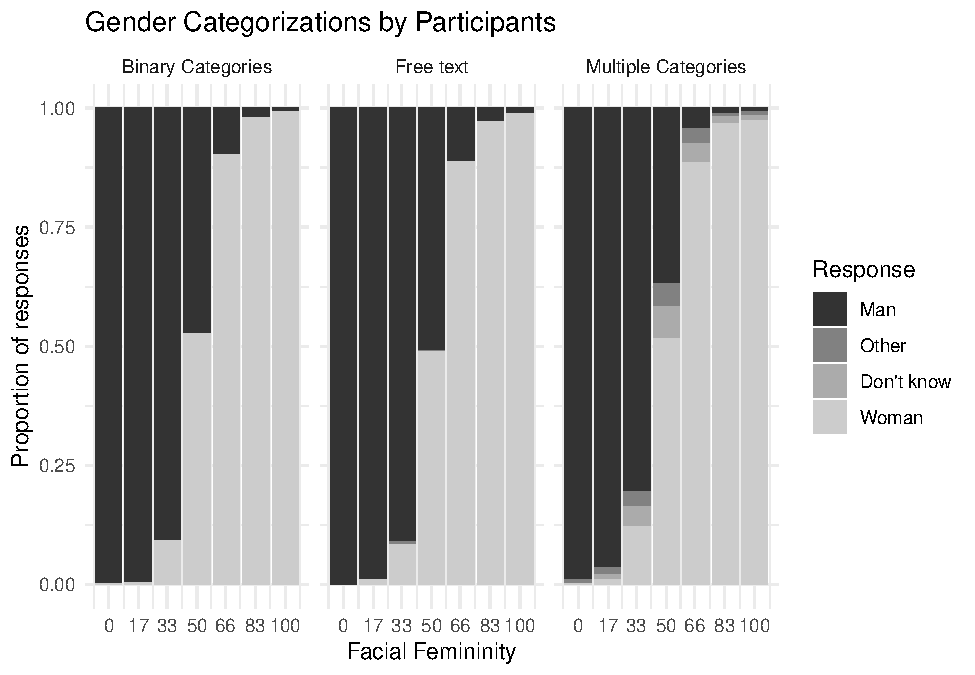
\includegraphics{resp_opts_manus23022_files/figure-latex/descriptives-1.pdf}
\caption{\label{fig:descriptives}Gender Categorizations by Participants}
\end{figure}

The first model was the Null model which included no additional predictors. The second was the Main Effects model which included unique intercepts for each pronoun condition and an overall effect of morph level. Lastly, the Interaction model included unique intercepts as well as unique slopes of morph level for each condition. For a detailed discussion of why this specification is preferred over the traditional dummy-variable approach, see McElreath (2020), but in short it ensures that the priors for each condition are the same, which is necessary for calculating Bayes Factors.

\begin{table}

\caption{\label{tab:loo}Relative predictive power of models describing the outcome on the categorization task}
\centering
\begin{threeparttable}
\begin{tabular}[t]{lcccc}
\toprule
  & LOO diff & St. Error diff & LOO & St. Error LOO\\
\midrule
Interaction & 0.00 & 0.00 & -234.17 & 23.23\\
Main Effect & -2.46 & 2.71 & -236.63 & 23.07\\
Null & -18.83 & 6.02 & -253.00 & 24.51\\
\bottomrule
\end{tabular}
\begin{tablenotes}[para]
\item \textit{Note.} 
\item LOO diff refers to the difference in loo between the model and the most predictive model. The first row describes the most predictive model, which is why the difference is 0
\end{tablenotes}
\end{threeparttable}
\end{table}

The models were compared using Leave-One-Out cross validation (Vehtari et al., 2017), a method for estimating a model's performance on out-of-sample data. This method of analyses produces LOO values which are not very informative of themselves, but when comparing models, lower values can be determined to show better predictive power. The results of model comparison are presented in Table~\ref{tab:loo}.
Table~\ref{tab:loo} suggests that the Interaction model is the most predictive, but the absolute differnce between the Interaction model and the Main effects model is small and more importantly, the difference is small in relation to the standard error of the difference. This suggests that the data is inconclusive about which model is most suitable. However, to test the specific question raised in the research question 1, we still carried on with the Interaction model.

\begin{figure}
\centering
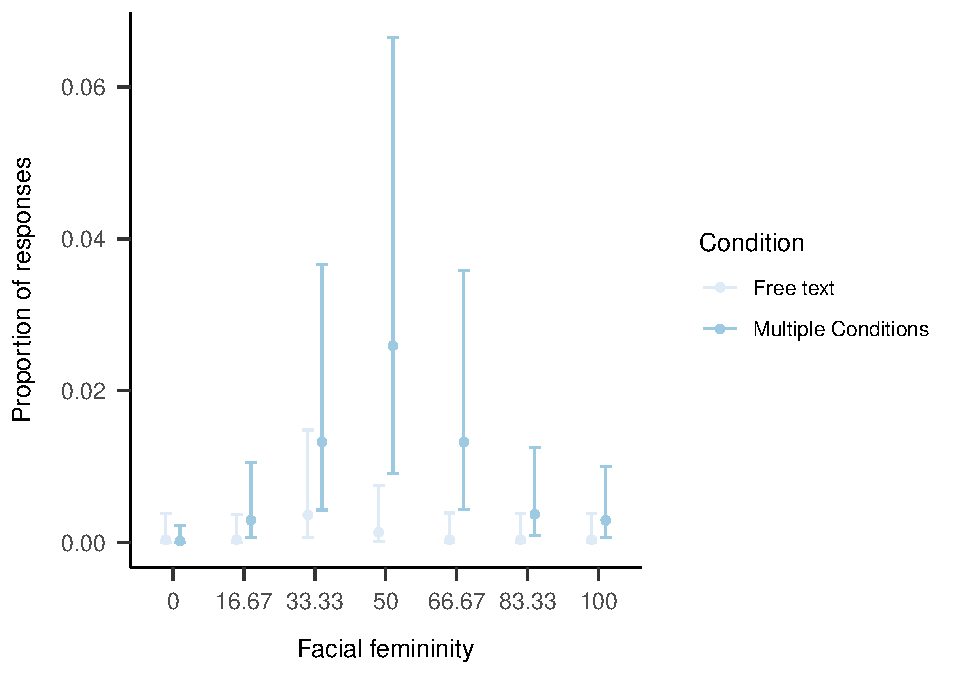
\includegraphics{resp_opts_manus23022_files/figure-latex/exp-one-inf-1.pdf}
\caption{\label{fig:exp-one-inf}Proportion of beyond-binary responses in the Mulitple categoreies and Free Text conditions}
\end{figure}

The estimates of the modelling are visualized in Figure~\ref{fig:exp-one-inf}. This again suggests that Three specific contrasts were tested with Bayes Factors calculated using the Savage-Dickey Density Ratio (ref). First, whether participants overall made more beyond-binary categorizations in the multiple categories condition than in the free text condition. The evidence suggests fairly convincingly that this is the case (Estimate = 0.02, CI ={[}0.00{]}, {[}0.18{]}, BF\textsubscript{10}= 97.67). Additionally, based on the curve in Figure~\ref{fig:exp-one-inf}, we explored whether the evidence supported this diference at morph level 50. The evidence was in favor of this differnce (Estimate = 0.02, CI ={[}0.00{]}, {[}0.20{]}, BF\textsubscript{10}= 17). Lastly, we tested the difference using quadratic weights, though here the difference was inconclusive (Estimate = 0.45, CI = {[}0.31{]} - {[}0.61{]}, BF\textsubscript{10}= 0.53). \emph{I'm not sure how to interpret this last finding}.

Overall, though, the evidence suggests at least somewhat strongly that when participants have the option of using beyond-binary response options, they use them.

\hypertarget{rq2-which-categories-replace-the-non-binary-options}{%
\subsection{RQ2: Which categories replace the non-binary options?}\label{rq2-which-categories-replace-the-non-binary-options}}

\begin{table}

\caption{\label{tab:rq2-table}Relative predictive power of models describing the outcome on the categorization task}
\centering
\begin{threeparttable}
\begin{tabular}[t]{llccc}
\toprule
  & LOO difference & St. Error diff & LOO & St. Error LOO\\
\midrule
morph\_only & 0.00 & 0.00 & -1343.71 & 43.17\\
main\_effects & -1.85 & 0.86 & -1345.56 & 43.17\\
condition\_only & -4.98 & 5.26 & -1348.69 & 44.49\\
Null & -5.36 & 4.88 & -1349.07 & 44.12\\
interaction & -6.69 & 3.02 & -1350.40 & 43.48\\
\bottomrule
\end{tabular}
\begin{tablenotes}[para]
\item \textit{Note.} 
\item LOO diff refers to the difference in loo between the model and the most predictive model. The first row describes the most predictive model, which is why the difference is 0
\end{tablenotes}
\end{threeparttable}
\end{table}

Based on the shape of Figure~\ref{fig:descriptives} it appears that ``man'' categorizations that are being crowded out by the beyond-binary options. To test whether this was actually the case, we carried out statistical analyses similar to the previous section, again using a mixed-effects model with random intercepts for participants and faces. To explore RQ2, we created three models, a Null model, a Main Effects model and an Interaction model. Similarly, these were then compared using LOO-CV. The results of this are presented in Table~\ref{tab:rq2-table}. This suggests that Interaction model is not the most predictive model, in fact it is the worst. Though, here again, we note that the standard error is quite high, suggesting the proper interpetation is rather that each model is roughly equally as predictive.

Based on the pattern in Figure~\ref{fig:descriptives} we did specifically test the contrast between the multiple categories condition and the other two conditions. The evidence were slightly in favor of there being no difference between the multiple categories and the free text conditions (Estimate = -0.49, CI ={[}-1.23{]}, {[}0.25{]}, BF\textsubscript{01}= 4.79) and moderately in favor of no difference between multiople categories and binary categories conditions (Estimate = -0.27, CI ={[}-0.99{]}, {[}0.45{]}, BF\textsubscript{01}= 9.08)

\hypertarget{discussion}{%
\subsection{Discussion}\label{discussion}}

The results from experiment 1 suggest that some participants do use the beyond-binary options when they have them, however only when these are explicitly spelled out. When participants are implicitly able to enter whatever they like, most still fell back on using woman/man. Furthermore, the results suggests that overall, even when participants used the beyond-binary options, this did not systematically affect their overall pattern of responses in terms of woman and man categorizations.

\hypertarget{experiment-2}{%
\section{Experiment 2}\label{experiment-2}}

\hypertarget{overview}{%
\subsection{Overview}\label{overview}}

The purpose of experiment 2 was primarily to test categorical perception. If categorical perception occurs, we would expect that scores of femininity to be lower than the percentage of femininity in the faces. Furthermore, if response options change perceptions of gender as a category, we would expect there to be less categorical perception in the multiple categories option.

\hypertarget{method-1}{%
\subsection{Method}\label{method-1}}

\hypertarget{participants-1}{%
\subsubsection{Participants}\label{participants-1}}

Participants (\emph{N} = 49) were speakers recruited through advertising online and on the university campus (\emph{M}\textsubscript{age}= 36.67, \emph{SD}\textsubscript{age} = 12.54). All participants were informed that participation was voluntary. In term of gender X women and Y men participated The participants were randomly allocated to conditions.

\hypertarget{stimuli-procedure}{%
\subsection{Stimuli \& Procedure}\label{stimuli-procedure}}

The stimuli and procedure for experiment 2 were identical to experiment 1. Experiment 2 differed only the response options conditions. For experiment 2, there response option conditions consisted of single dimension, which ranged from ``woman'' to ``man'' and ``multiple dimension'' which ranged from ``not woman'' to ``woman'' and ``not man'' to ``man''. For the multiple dimensions condition, participants rated the same faces according to both scales, but on separate trials.

\hypertarget{results-1}{%
\section{Results}\label{results-1}}

The mean ratings in both conditions are presented in Figure~\ref{fig:descriptives-two}.

\begin{figure}
\centering
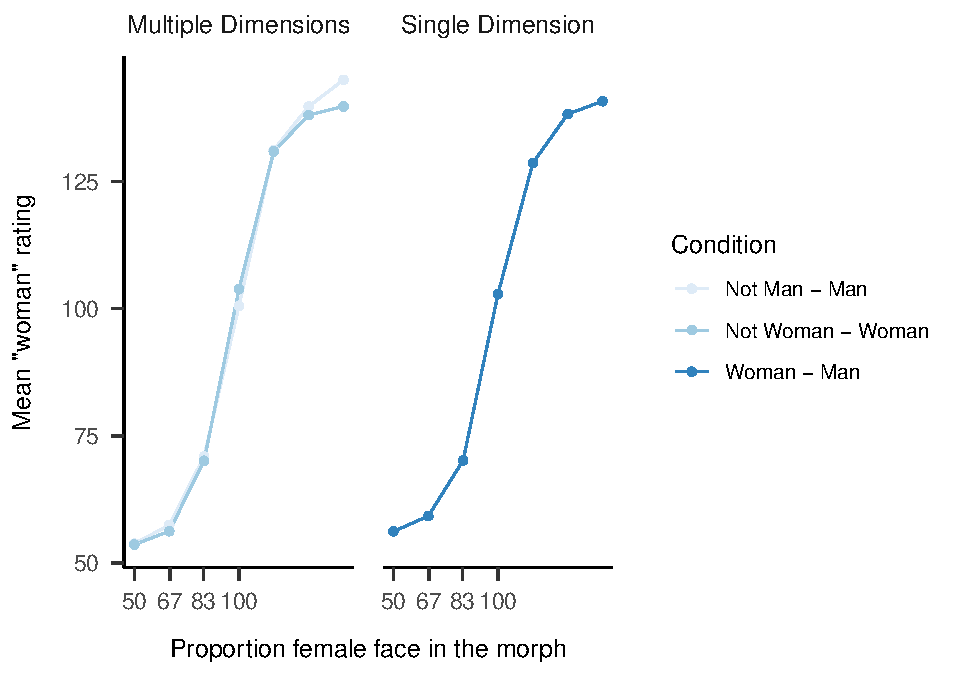
\includegraphics{resp_opts_manus23022_files/figure-latex/descriptives-two-1.pdf}
\caption{\label{fig:descriptives-two}Mean ratings of faces in Single dimension and multiple dimensions}
\end{figure}

As a further test of the research question, we also fitted the data to a Bayesian mixed effects model, with participants and faces modeled as random intercepts. Additionally, the morph levels were entered as categorical predictors, rather than as continuous variables. Similar to study 1, the initial approach consisted of several models which were compared against each other using LOO-CV. Again, the models were a Null model, with no additional predictors, a Main Effects model with main effects of morph level and condition, but no interaction, and a Interaction model (for complete model specification, see the Supplementary material.)

\begin{figure}
\centering
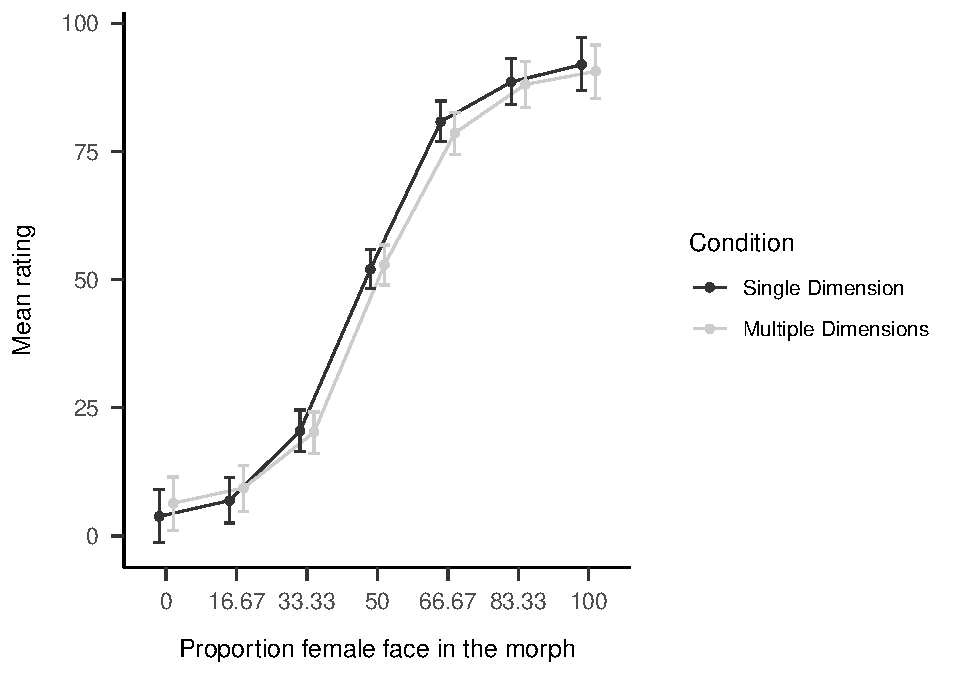
\includegraphics{resp_opts_manus23022_files/figure-latex/exp-two-inf-1.pdf}
\caption{\label{fig:exp-two-inf}Mean gender ratings in Single Dimension and Multiple Dimensions conditions}
\end{figure}

Based on the results of LOO-CV, we continued with the Interaction model. We carried out two comparisions. The first was a quadratic contrasts \emph{which I have still to carry out}. Because the critical levels where we might expect to see a differ, we also compared the mean rating at 33.33 morph and at 66.67 morph. At 33.33 the evidence strongly suggested that the two conditions are the same
(Estimate = 0.28, CI ={[}-3.91{]}, {[}4.51{]}, BF\textsubscript{01}= 31.57). This was also the case at 66.67
(Estimate = 2.29, CI ={[}-2.03{]}, {[}6.57{]}, BF\textsubscript{01}= 19.17). Overall, both conditions showed fairly strong tendencies toward categorical perception and they did not differ in this regard.

\hypertarget{discussion-1}{%
\section{Discussion}\label{discussion-1}}

Experiment 2 was designed to test whether response options which did not present women and men as opposing categories changed participants categorical perception. Overall, the results indicated that in terms of categorical perception, the two conditions were very similar, suggesting that the binary view of language is very strong and that participants do not change their view of gender depending on

\hypertarget{overall-discussion}{%
\section{Overall discussion}\label{overall-discussion}}

Overall, some important findings emerged from this experiment. First, there was strong evidence that participants will use beyond-binary actions to categorize faces, if given the options. It is also clear that providing these options do not change the overall distributions of scores

\newpage

\hypertarget{references}{%
\section{References}\label{references}}

\hypertarget{refs}{}
\begin{CSLReferences}{1}{0}
\leavevmode\vadjust pre{\hypertarget{ref-R-papaja}{}}%
Aust, F., \& Barth, M. (2022). \emph{{papaja}: {Prepare} reproducible {APA} journal articles with {R Markdown}}. \url{https://github.com/crsh/papaja}

\leavevmode\vadjust pre{\hypertarget{ref-R-tinylabels}{}}%
Barth, M. (2022). \emph{{tinylabels}: Lightweight variable labels}. \url{https://cran.r-project.org/package=tinylabels}

\leavevmode\vadjust pre{\hypertarget{ref-R-brms_a}{}}%
Bürkner, P.-C. (2017). {brms}: An {R} package for {Bayesian} multilevel models using {Stan}. \emph{Journal of Statistical Software}, \emph{80}(1), 1--28. \url{https://doi.org/10.18637/jss.v080.i01}

\leavevmode\vadjust pre{\hypertarget{ref-R-brms_b}{}}%
Bürkner, P.-C. (2018). Advanced {Bayesian} multilevel modeling with the {R} package {brms}. \emph{The R Journal}, \emph{10}(1), 395--411. \url{https://doi.org/10.32614/RJ-2018-017}

\leavevmode\vadjust pre{\hypertarget{ref-R-brms_c}{}}%
Bürkner, P.-C. (2021). Bayesian item response modeling in {R} with {brms} and {Stan}. \emph{Journal of Statistical Software}, \emph{100}(5), 1--54. \url{https://doi.org/10.18637/jss.v100.i05}

\leavevmode\vadjust pre{\hypertarget{ref-R-gcookbook}{}}%
Chang, W. (2018). \emph{Gcookbook: Data for "r graphics cookbook"}. \url{https://CRAN.R-project.org/package=gcookbook}

\leavevmode\vadjust pre{\hypertarget{ref-R-Rcpp_b}{}}%
Eddelbuettel, D., \& Balamuta, J. J. (2018). {Extending extit{R} with extit{C++}: A Brief Introduction to extit{Rcpp}}. \emph{The American Statistician}, \emph{72}(1), 28--36. \url{https://doi.org/10.1080/00031305.2017.1375990}

\leavevmode\vadjust pre{\hypertarget{ref-R-Rcpp_a}{}}%
Eddelbuettel, D., \& François, R. (2011). {Rcpp}: Seamless {R} and {C++} integration. \emph{Journal of Statistical Software}, \emph{40}(8), 1--18. \url{https://doi.org/10.18637/jss.v040.i08}

\leavevmode\vadjust pre{\hypertarget{ref-R-bayesplot}{}}%
Gabry, J., Simpson, D., Vehtari, A., Betancourt, M., \& Gelman, A. (2019). Visualization in bayesian workflow. \emph{J. R. Stat. Soc. A}, \emph{182}, 389--402. \url{https://doi.org/10.1111/rssa.12378}

\leavevmode\vadjust pre{\hypertarget{ref-R-tidybayes}{}}%
Kay, M. (2022). \emph{{tidybayes}: Tidy data and geoms for {Bayesian} models}. \url{https://doi.org/10.5281/zenodo.1308151}

\leavevmode\vadjust pre{\hypertarget{ref-R-base}{}}%
R Core Team. (2022). \emph{R: A language and environment for statistical computing}. R Foundation for Statistical Computing. \url{https://www.R-project.org/}

\leavevmode\vadjust pre{\hypertarget{ref-R-ggplot2}{}}%
Wickham, H. (2016). \emph{ggplot2: Elegant graphics for data analysis}. Springer-Verlag New York. \url{https://ggplot2.tidyverse.org}

\leavevmode\vadjust pre{\hypertarget{ref-R-dplyr}{}}%
Wickham, H., François, R., Henry, L., \& Müller, K. (2022). \emph{Dplyr: A grammar of data manipulation}. \url{https://CRAN.R-project.org/package=dplyr}

\leavevmode\vadjust pre{\hypertarget{ref-R-tidyr}{}}%
Wickham, H., \& Girlich, M. (2022). \emph{Tidyr: Tidy messy data}. \url{https://CRAN.R-project.org/package=tidyr}

\end{CSLReferences}


\end{document}
